\documentclass{beamer}
\usepackage{setspace}
\usepackage{bm,color,float,epstopdf,amsthm,epstopdf}
\usepackage{multirow,tikz}
\newcommand{\fttheory}[1]{\fcolorbox{blue}{blue}{\color{white}\textbf{#1}\hspace{\textwidth}}}
\newcommand{\ftexampl}[1]{\fcolorbox{orange}{orange}{\color{black}\textbf{#1}\hspace{\textwidth}}}
\newcommand{\ftdata}[1]{\fcolorbox{violet}{violet}{\color{white}\textbf{#1}\hspace{\textwidth}}}
\newcommand{\ftheader}[1]{\fcolorbox{lightgray}{lightgray}{\color{black}\textbf{#1}\hspace{\textwidth}}}
\newcommand{\ftvocab}[1]{\fcolorbox{cyan}{cyan}{\color{black}\textbf{#1}\hspace{\textwidth}}}
\newcommand{\usd}{\text{ {\scriptsize USD}}}
\newcommand{\eur}{\text{ {\scriptsize EUR}}}
\newcommand{\aud}{\text{ {\scriptsize AUD}}}
\newcommand{\mxn}{\text{ {\scriptsize MXN}}}
\newcommand{\musd}{\text{ m {\scriptsize USD}}}
\newcommand{\meur}{\text{ m {\scriptsize EUR}}}
\newcommand{\maud}{\text{ m {\scriptsize AUD}}}

\renewcommand{\arraystretch}{1.5}
\begin{document}

%-----------------------------------------------------------------------------%
% fowards
\begin{frame}{\ftheader{Fowards}}
	\begin{itemize}
		\item In this lecture, we begin our study of derivatives 
		\item We will start with \textit{forwards} 
		\item Standardized implementations of forwards are called \textit{futures}
		\item Henceforth, I will refer to everything as a ``forward''
		\item We will then use forwards to study\\
			(1) swaps\\ 
			(2) exchange rates
	\end{itemize}
\end{frame}

%-----------------------------------------------------------------------------%
% vocabulary
\begin{frame}{\ftvocab{Vocabulary}}
	\begin{itemize}
		\item A \textit{derivative} is a security whose payoff depend on the payoff of other securities
		\item A \textit{forward} is a contract that requires future delivery of asset at agreed-upon price
		\item \textit{Cash settlement} means delivering the cash value of the underlying asset (rather than the asset itself) to satisfy the contract
		\item The \textit{underlying} security (stock, bond, currency, commodity) on which the forward is written
		\item The \textit{future price} is the agreed-upon price to be paid on a futures contract at maturity
		\item The \textit{spot price} is the actual market price of the security 
	\end{itemize}
\end{frame}

%-----------------------------------------------------------------------------%
% strategies
\begin{frame}{\fttheory{Mechanics}}
	\begin{itemize}
		\item If you are \textit{long} a forward, then you commit to \textit{sell} the security, while if you are short, you commit to \textit{buy} the security
		\item With cash settlement, the party who is short does not have to literally sell the underlying security to her counterparty; rather, she can just pay her counterparty the difference between the spot price and the future price in cash
		\item Since positions are settled at maturity, there is no initial cash flow: everything happens ``in the future''
    \end{itemize}
\end{frame}

%-----------------------------------------------------------------------------%
% payoffs
\begin{frame}{\fttheory{Forward Payoffs}}
    \begin{center}
        \begin{tabular}{cc}
            Long Forward: $S-K$ & Short Forward: $K-S$ \\
            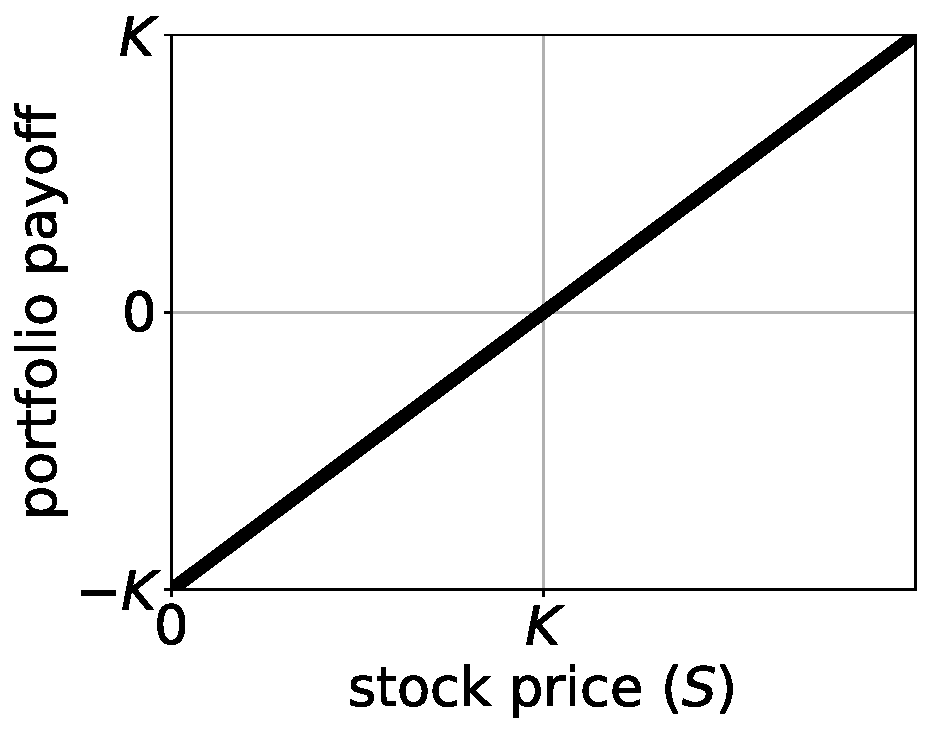
\includegraphics[scale=.3]{longforward} & 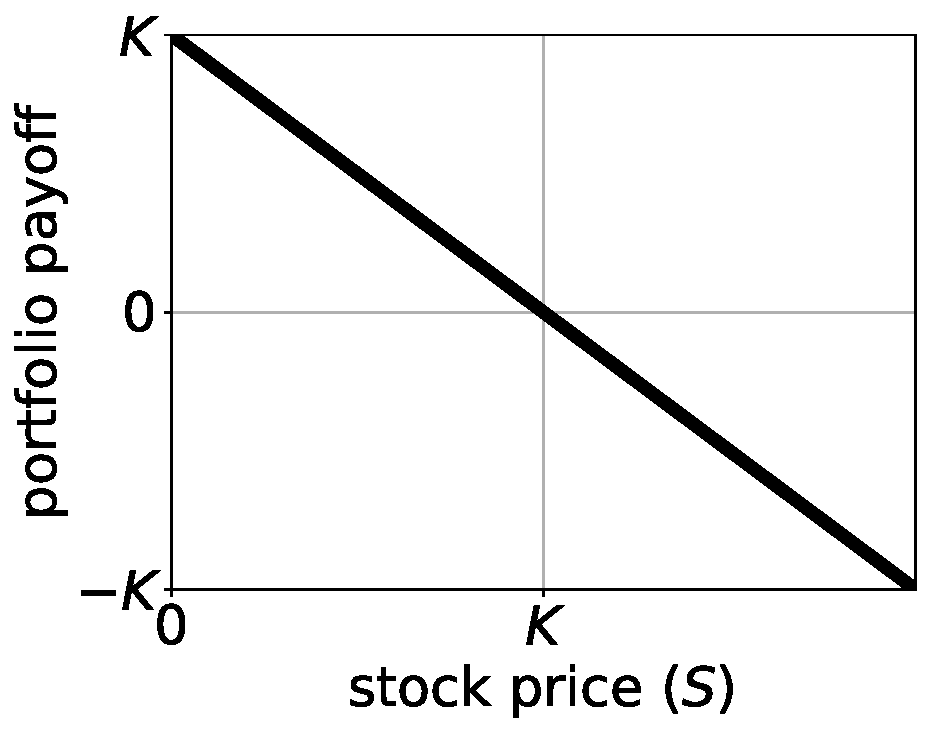
\includegraphics[scale=.3]{shortforward}
        \end{tabular}
    \end{center}
	\begin{itemize}
		\item The trader in the long position is said to ``buy'' a contract; the short-side trader ``sells'' a contract. 
        \item Basis: difference between futures price and spot price $K-S$
	\end{itemize}
\end{frame}

%-----------------------------------------------------------------------------%
% payoffs
\begin{frame}{\ftexampl{\hypertarget{frame:payoffs1}{Forward Payoffs: Problem 1}}}
	\textbf{Problem.} Suppose Apple (AAPL) trades for $270\usd$. James Simons (Renaissance Technologies) is going to write a 3-year 
\end{frame}

%-----------------------------------------------------------------------------%
% corporate applications: a vignette
\begin{frame}{\fttheory{Corporate Applications: a Vignette}}
	\begin{itemize}
		\item Consider an oil company and an airline.  
		\item How much will the price of oil be in the future, when they are ready to sell the oil they produced?  
		\item The revenue of this company depends on oil prices, which are extremely volatile.
		\item The airline has a problem that mirrors that of the oil production company. 
		\item How can forwards help these two firms?
	\end{itemize}
\end{frame}

%-----------------------------------------------------------------------------%
% corporate applications: a vignette
\begin{frame}{\fttheory{Corporate Applications: a Vignette}}
	\begin{itemize}
		\item The two firms can enter into an agreement today that specifies the price at which the oil producer sells the oil to the other company in the future. 
		\item Such an agreement will reduce the source of risk for both parties!  
		\item The oil producer delivers oil at a price agreed upon now, regardless of the market price at the time when oil is produced. 
		\item This requires that both parties be willing to lock in the price to be paid or received for delivery of the commodity. 
		\item This can be achieved using forwards.
	\end{itemize}
\end{frame}

%-----------------------------------------------------------------------------%
% corporate applications
\begin{frame}{\ftdata{Corporate Applications}}
    \begin{center}
        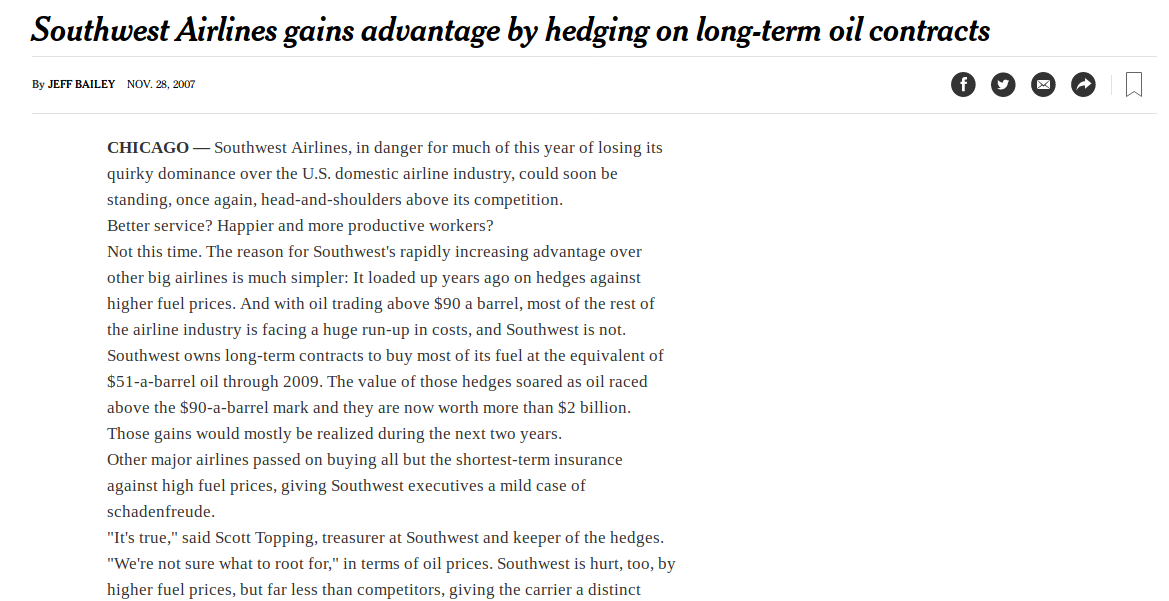
\includegraphics[scale=.3]{swa}
    \end{center}
\end{frame}

%-----------------------------------------------------------------------------%
% pricing new forwards
\begin{frame}{\fttheory{Spot-Futures Parity}}
\begin{itemize}
	\item Having looked at the mechanics and applications of forwards, we know consider their pricing
	\item $T$ is the term, $S_{0}$ is the spot price on date $0$, $S_{T}$ is the spot price on date $T$, and $K$ is the future price
    \item Spot-Futures Parity $K\overset{\text{``should''}}{=}S_{0}(1+r_{F})^{T}$
\end{itemize}
    \begin{center}
        \begin{tabular}{lccc}
            Security & Q & CF$_{0}$ & CF$_{T}$ \\ \hline
            Forward & 1 & 0 & $S_{T}-K$ \\ \hline\hline
            Stock & 1 & $-S_{0}$ & $S_{T}$ \\
			Risk-Free & $-K/(1+r_{F})^{T}$ & $K/(1+r_{F})^{T}$ & $-K$ \\ \hline
			& & $-S_{0}+K/(1+r_{F})^{T}$ & $S_{T}-K$
        \end{tabular}
    \end{center}
\end{frame}

%-----------------------------------------------------------------------------%
% pricing new forwards
\begin{frame}{\ftexampl{\hypertarget{frame:spotfuturesparityhedging}{Spot-Futures Parity: Hedging Problem}}}
	\textbf{Problem:} You're in sales at Goldman Sachs. A client wants a five-year forward on 1\musd of Apple, which currently sells for 270\usd. The annually compounded risk-free rate is .25\%. What should the price $K$ be? How do you hedge the position?\\

 \textbf{Solution:} The futures price is
	\begin{equation}
		K=S_{0}(1+r_{F})^{T}=(1\musd)(1+.0025)^{5}=1.0126\musd
	\end{equation}
	This means that in five years, Goldman Sachs is obligated to sell the client $(1\musd/270\usd)=$ shares of Apple for a total of 1.0136\musd. In order to hedge this transaction, Goldman Sachs can buy
\end{frame}

%-----------------------------------------------------------------------------%
% pricing new forwards
\begin{frame}{\ftexampl{\hypertarget{frame:spotfuturesparitymargin}{Spot-Futures Parity: Margin Problem}}}
	\textbf{Motivation.} Because both parties to a futures contract are exposed to losses, both must post margins.\\

	\textbf{Problem.} Suppose that you buy a one-year forward on 10k shares of SPY, which currently sells for 275\usd. The risk-free rate is .25\%. You are required to post an initial margin of 50\%.  \begin{enumerate}
		\item What should the forward price be? 
		\item How much margin (USD) must you post?  
		\item If SPY drops by 5\% tomorrow, what will the new forward price be (approximately)?           
		\item How much margin do you have left? 
		\item What is your return?
	\end{enumerate}
\end{frame}

%-----------------------------------------------------------------------------%
% pricing new forwards
\begin{frame}{\ftexampl{Spot-Futures Parity: Margin Problem}}
	\textbf{Solution.} 
	\begin{enumerate}
		\item The forward price (per share) is
			\begin{equation}\small
				K=S_{0}(1+r_{F})^{T}=(275\usd)(1+.0025)=275.6875\usd
			\end{equation}
		\item You must post 
		\item Suppose that SPY drops by 5\% tomorrow: $S_{0}=(95\%)(275\usd)=261.25\usd$. If ignoring the 1 day that has past, 
			\begin{equation}\small
				K=S_{0}(1+r_{F})^{T}=(261.25\usd)(1+.0025)=261.9031\usd
			\end{equation}
		\item How much margin do you have left? 
		\item What is your return?
	\end{enumerate}
\end{frame}

%-----------------------------------------------------------------------------%
% pricing existing forwards
\begin{frame}{\fttheory{Pricing Existing Forwards}}
   \begin{itemize}
	   \item Forwards, like all of the derivatives we will study, can be sold in a secondary market
       \item Suppose you go long a forward that expires in \underline{two} years.
       \item Step forward one year. 
       \item Consider a new forward that expires in \underline{one} year.
       \item How much could you sell your old forward for (say $f_{0}$)? 
	   \item This is the problem of pricing an existing forward
   \end{itemize}
\end{frame}

%-----------------------------------------------------------------------------%
% pricing existing forwards
\begin{frame}{\fttheory{Pricing Existing Forwards}}
    How do you price anything? Build a replicating portfolio!
    \begin{center}
        \begin{tabular}{lcc}
            Security & CF$_{1}$ & CF$_{2}$ \\ \hline
            Old Forward ($K_{0}$) &  $-f_{0}$ & $S_{2}-K_{0}$ \\ \hline
            \multicolumn{3}{c}{Replicating Portfolio} \\ \hline
			New Forward ($K_{1}$) & $0$& $S_{2}-K_{1}$ \\ 
			Risk Free &  $-(K_{1}-K_{0})/(1+r_{F})$ & $K_{1}-K_{0}$ \\ \hline
			& $-(K_{1}-K_{0})/(1+r_{F})$ & $S_{2}-K_{0}$
        \end{tabular}
    \end{center}
    \begin{equation}
		\boxed{f_{0}\overset{\text{``should''}}{=}\frac{K_{1}-K_{0}}{1+r_{F}}}
    \end{equation}
\end{frame}

%-----------------------------------------------------------------------------%
% pricing existing forwards: problem 1
\begin{frame}{\ftexampl{\hypertarget{frame:pricingexistingforwards1}{Pricing Existing Forwards: Problem 1}}}
	\textbf{Problem.} Suppose that the stock price was $S_{0}=100\usd$ a year ago and the stock price is $S_{1}=101.50\usd$ today. What is the future price of a two-year forward written a year ago? Suppose that the annually compounded risk-free rate is $r_{F}=1.5\%$\\
	\vfill
	\textbf{Solution.}
	\begin{itemize}
        \item The old and new forward prices are 
            \begin{align}
				K_{0}&=S_{0}(1+r_{F})^{2}=121\usd\\
				K_{1}&=S_{1}(1+r_{F})=126\usd
            \end{align}
        \item The old forward trades now trades for
            \begin{equation}
				f_{0}=\frac{K_{1}-K_{0}}{1+r_{F}}=\frac{126\usd-121\usd}{1+.1}=4.54\usd
            \end{equation}
    \end{itemize}
\end{frame}

%-----------------------------------------------------------------------------%
% pricing existing forwards: problem 2
\begin{frame}{\ftexampl{\hypertarget{frame:pricingexistingforwards2}{Pricing Existing Forwards: Problem 2}}}
	\textbf{Problem.} $S_{0}=100\usd$, $S_{1}=110\usd$, $r=10\%$\\
	\vfill
	\textbf{Solution.}
    \begin{itemize}
		\item The old and new forward prices are 
            \begin{align}
				K_{0}&=S_{0}(1+r_{F})^{2}=121\usd\\
				K_{1}&=S_{1}(1+r_{F})=121\usd
            \end{align}
        \item The old forward trades for
            \begin{equation}
				f_{0}=\frac{K_{1}-K_{0}}{1+r_{F}}=\frac{121\usd-121\usd}{1+.1}=0\usd
            \end{equation}
    \end{itemize}
\end{frame}

%-----------------------------------------------------------------------------%
% application i: swaps
\begin{frame}{\ftheader{Application I: Swaps}}
	\begin{itemize}
		\item A swap is a contract in which parties ``swap'' cash-flows. 
		\item Party $A$ has cash flows $c_{1}^{A},c_{2}^{A},\ldots$
		\item Party $B$ has cash flows $c_{1}^{B},c_{2}^{B},\ldots$
		\item $A$ and $B$ swap: $B$ pays $A$ $c_{1}^{B},c_{2}^{B},\ldots$ and $A$ pays $B$ $c_{1}^{A},c_{2}^{A},\ldots$
		\item Swaps are technically portfolios of forwards
	\end{itemize}
\end{frame}

%-----------------------------------------------------------------------------%
% swaps: ibm and the world bank
\begin{frame}{\ftdata{Swaps: IBM and the World Bank}}
    \begin{itemize}
        \item Salomon Brothers wrote the first swap in 1981
        \item The World Bank is an international organization that borrows from developed countries and lends to developing countries
        \item In 1981, Swiss debt was cheap, so the World Bank wanted to borrow there, but...
        \item Switzerland limited how much the World Bank could borrow
        \item IBM had already borrowed in Switzerland and wanted dollars
        \item Salomon proposed ``swapping'' cash flows
        \item The World Bank borrowed dollars
        \item IBM paid the World Bank's dollar obligations
        \item The World Bank paid IBM's franc obligations
        \item It was as if the World Bank borrowed in francs and IBM borrowed in dollars
    \end{itemize}
\end{frame}

%-----------------------------------------------------------------------------%
% swaps: pricing
\begin{frame}{\fttheory{Swaps: Pricing}}
    \begin{itemize}
        \item $A$ borrows $p_{A}$, pays coupon $c_{A}$ each period
        \item $B$ borrows $p_{B}$, pays coupon $c_{B}$ each period
    \end{itemize}
\begin{center}
\begin{tikzpicture}
    
	\draw (0,0) -- (4.5,0) node[anchor=west]{$\cdots$};
    \foreach \x in {0,2,4}
    \draw(\x,-.1) -- (\x, .1);
    \draw (0,0) node[above=3pt] {0};
    \draw (2,0) node[above=3pt] {1};
    \draw (4,0) node[above=3pt] {2};
    \draw (-2,0) node[] {Firm $B$};
    \draw (0,0) node[below=3pt] {$p_{B}$};
    \draw (2,0) node[below=3pt] {$-c_{B}$};
    \draw (4,0) node[below=3pt] {$-c_{B}$};
    
    \draw (0,2) -- (4.5,2) node[anchor=west]{$\cdots$};
    \foreach \x in {0,2,4}
    \draw(\x,1.9) -- (\x,2.1);
    \draw (0,2) node[above=3pt] {0};
    \draw (2,2) node[above=3pt] {1};
    \draw (4,2) node[above=3pt] {2};
    \draw (-2,2) node[] {Firm $A$};
    \draw (0,2) node[below=3pt] {$p_{A}$};
    \draw (2,2) node[below=3pt] {$-c_{A}$};
    \draw (4,2) node[below=3pt] {$-c_{A}$};

\end{tikzpicture}
\end{center}
	\begin{itemize}
		\item If the loans are priced correctly, then for rates $r_{A}$ and $r_{B}$,
		\begin{align}
			p_{A}&=\frac{c_{A}}{1+r_{F}}+\frac{c_{A}}{(1+r_{F})^{2}}+\cdots\\
			p_{B}&=\frac{c_{B}}{1+r_{F}}+\frac{c_{B}}{(1+r_{F})^{2}}+\cdots
		\end{align}
	\end{itemize}
\end{frame}

%-----------------------------------------------------------------------------%
% interest rate swaps
\begin{frame}{\fttheory{Interest Rate Swaps}}
    $w_{0}$ is the price of the swap
    \begin{center}
        \begin{tabular}{lccc}
            Security &  CF$_{0}$ & CF$_{1}$ & CF$_{2}$\\ \hline
            \multicolumn{4}{c}{\textbf{Firm A}} \\ \hline
            Loan & $+p_{A}$ & $-c_{A}$ & $-c_{A}$\\
            Swap & $-w_{0}$ & $c_{A}-c_{B}$ & $c_{A}-c_{B}$ \\ \hline
            & $p_{A}-w_{0}$ & $-c_{B}$ & $-c_{B}$ \\ \hline
            \multicolumn{4}{c}{\textbf{Firm B}} \\ \hline
            Loan & $+p_{B}$ & $-c_{B}$ & $-c_{B}$ \\
            Swap & $+w_{0}$ & $-(c_{A}-c_{B})$ & $-(c_{A}-c_{B})$ \\ \hline
            & $p_{B}+w_{0}$ & $-c_{A}$ & $-c_{A}$
        \end{tabular}
    \end{center}
\end{frame}

%-----------------------------------------------------------------------------%
% interest rate swaps
\begin{frame}{\fttheory{Interest Rate Swaps: Pricing}}
    $w_{0}$ is the price of the swap
    \begin{center}
        \begin{tabular}{lccc}
            Security & CF$_{0}$ & CF$_{1}$ & CF$_{2}$\\ \hline
            Swap & $-w_{0}$ & $c_{A}-c_{B}$ & $c_{A}-c_{B}$ \\ \hline
            \multicolumn{4}{c}{Replicating Portfolio} \\ \hline
            Loan $A$ & $-p_{A}$ & $+c_{A}$ & $+c_{A}$ \\ 
            Loan $B$ & $+p_{B}$ & $-c_{B}$ & $-c_{B}$ \\ \hline
            & $-p_{A}+p_{B}$ & $c_{A}-c_{B}$ & $c_{A}-c_{B}$
        \end{tabular}
    \end{center}
    \begin{equation}
        \boxed{w_{0}\overset{\text{``should''}}{=}p_{A}-p_{B}}
    \end{equation}
\end{frame}

%-----------------------------------------------------------------------------%
% interest rate swaps: problem
\begin{frame}{\ftexampl{\hypertarget{frame:interestrateswaps}{Interest Rate Swaps: Problem}}}
    Suppose that the yield on a one-year bond is 5\% ($_{0}y_{1}=5\%$) and the yield on a two-year bond is 10\% ($_{0}y_{2}=10\%$). What should the swap trade for ($w_{0}$)? 
\end{frame}

%-----------------------------------------------------------------------------%
% application ii: exchange rates
\begin{frame}{\ftheader{Application II: Exchange Rates}}
	\begin{itemize}
		\item International finance is a large and rich topic
		\item Today, we're going to price currencies
		\item We're going to study a couple of practical examples
        \item Currencies are like tacos
        \item I go to 3 Amigos and buy tacos, I go to Chase and buy pesos
        \item In both cases, I pay with dollars
        \item Let $E$ denote the price of foreign currency
		\item E.g. a Mexican peso sells for $E=.04$ \text{USD}
    \end{itemize}
\end{frame}

%-----------------------------------------------------------------------------%
% interest rate parity
\begin{frame}{\fttheory{Interest Rate Parity}}
    \begin{itemize}
        \item Two countries, domestic ($D$) and foreign ($F$), $r_{D}$ is the risk-free rate in $D$, $r_{F}$ in $F$, $E_{0}$ is the spot price of $F$'s currency, and $K_{0}$ is the price of a forward on $F$'s currency
		\item \textit{Interest Rate Parity} occurs when
            \begin{equation}
				\boxed{1+r_{D}=(1+r_{F})\cdot\frac{K_{0}}{E_{0}}}
            \end{equation}
		\item Put differently, you should not be able to make more money on a Euro denominated risk-free asset (e.g. German bunds) than on a Dollar denominated risk-free asset (e.g. US Treasuries)
    \end{itemize}
\end{frame}

%-----------------------------------------------------------------------------%
% interest rate parity: problem
\begin{frame}{\ftexampl{\hypertarget{frame:interestrateparity}{Interest Rate Parity: Problem}}}
	\textbf{Problem.} $1\aud$ costs $E_{0}=.64\usd$. The yields on 1-year Australianand US government bonds are .245\% and .3\% respectively. What should the 1-year forward price of $1\aud$ be? If the 1-year forward price of $1\aud$ is $K_{0}=.6402\usd$, what arbitrage opportunity is available to you?\\ 
\vfill
	\textbf{Solution.} Let's first compute what the forward price should be under Interest Rate Parity:
	\begin{equation}
		K_{0}=\frac{1+r_{D}}{1+r_{F}}\cdot E_{0}=\frac{1+.00300}{1+.00245}(.64\usd)=.6404\usd
	\end{equation}
	As you can see, the 1-year forward price is $.6402\usd$ is less than what it should be under Interest Rate Parity, so we want to \underline{borrow} AUD and \underline{lend} USD.
\end{frame}

%-----------------------------------------------------------------------------%
% interest rate parity: problem
\begin{frame}{\ftexampl{Interest Rate Parity: Problem}}
	\textbf{Solution (continued).} To exploit the arbitrage opportunity, use the following procedure.\\
	\vfill
	Today, 
	\begin{enumerate}
		\item borrow $1\maud$, 
		\item buy $1\maud\times(.64\usd\:/\aud)=.64\musd$
		\item buy $.64\musd$ of US government bonds
		\item sell a 1-year forward for $.6402\usd$
	\end{enumerate}
	In one year, 
	\begin{enumerate}
		\item collect $(1+.003)\times(.64\musd)=.6419\musd$
		\item $.6419\musd\:/(.6402\usd\:/\aud)=1.0027\maud$
		\item repay $1\maud\times(1+.00245)=1.0025\maud$ 
		\item you have collected a profit of $.0002\maud$ (about $200\aud$)
	\end{enumerate}
\end{frame}

%-----------------------------------------------------------------------------%
% irp vs. ppp
\begin{frame}{\ftexampl{Interest Rate Parity vs. Purchasing Power Parity}}
	\begin{itemize}
		\item Can we apply the same logic to other assets?
		\item \textit{Purchasing power parity} refers to the ability to buy the same basket of goods/services around the world for the same price
        \item A taco in the US sells for $3\usd$, a taco in Mexico sells for $20\mxn$, a peso sells for $.05\usd$. What arbitrage opportunity is available to you?
        \item Buy $20\mxn$ for $1\usd$, buy 1 taco in Mexico for 20$\mxn$, sell 1 taco in the US for $3\usd$. You've made $2\usd$.
		\item Money can be moved around the world (almost) costlessly. Tacos cannot.
    \end{itemize}
\end{frame}

%-----------------------------------------------------------------------------%
% the economist's big-mac index
% TODO: eventually, I'd like to do bigmac on one side, interest rates on other
\begin{frame}{\ftdata{The Economist's Big-Mac Index}}
    \begin{center}
        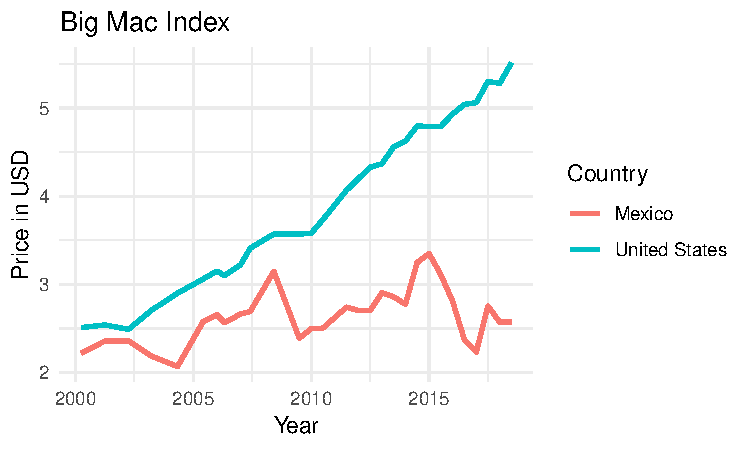
\includegraphics[scale=.75]{bigmac}
    \end{center}
	\noindent Although interest rate partity tends to hold in the data, does not. This is call the Penn effect and it is due to (1) limits to arbitrage and (2) differences in economic development. \\
\end{frame}

\begin{frame}{\ftexampl{Problems}}
	\begin{enumerate}
		\item \hyperlink{frame:payoffs1}{Forward Payoffs: Problem 1}
		\item \hyperlink{frame:spotfuturesparityhedging}{Spot-Futures Parity: Hedging Problem}
		\item \hyperlink{frame:spotfuturesparitymargin}{Spot-Futures Parity: Margin Problem}
		\item \hyperlink{frame:pricingexistingforwards1}{Pricing Existing Forwards: Problem 1}
		\item \hyperlink{frame:pricingexistingforwards2}{Pricing Existing Forwards: Problem 2}
		\item \hyperlink{frame:interestrateswaps}{Interest Rate Swaps: Problem}
		\item \hyperlink{frame:interestrateparity}{Interest Rate Parity: Problem}
	\end{enumerate}
\end{frame}
\end{document}
